\documentclass[10pt, conference, compsocconf]{IEEEtran}

% ACM-style
%\documentclass{sig-alternate}

%%%%%%%%%%%%%%%%%%%%%%%%%%%%%%%%%%%%%%%%%%%%%%%%%%%%%%%%%%%%%%%%%%%%%%%%%%%%%%%

% Hacks to revert the changes IEEEtran makes to table caption styles

\usepackage{etoolbox}

\makeatletter
\patchcmd{\@makecaption}
  {\scshape}
  {}
  {}
  {}
\makeatother

%%%%%%%%%%%%%%%%%%%%%%%%%%%%%%%%%%%%%%%%%%%%%%%%%%%%%%%%%%%%%%%%%%%%%%%%%%%%%%%

\usepackage{lmodern}
\usepackage{amsmath}
\usepackage{amsfonts}
\usepackage[hidelinks]{hyperref}
\usepackage{cite}

\usepackage{color}

\usepackage{graphicx}  % \includegraphics
\usepackage{multirow}  % \multicolumn, \multirow
\usepackage{subfig}    % \subfloat

% Place subfigure captions on top
\captionsetup[subfigure]{position=top}

% Make figure labels bold
\captionsetup[figure]{labelfont=bf}

%%%%%%%%%%%%%%%%%%%%%%%%%%%%%%%%%%%%%%%%%%%%%%%%%%%%%%%%%%%%%%%%%%%%%%%%%%%%%%%

% Highlighted source code listings

\usepackage{listings}
\lstloadlanguages{C++}

\lstset{
language=C++,                       % choose the language of the code
basicstyle=\footnotesize\ttfamily,  % the size of the fonts that are used for the
                                    % code
numbers=none,                       % where to put the line-numbers
numberstyle=\tiny,                  % the size of the fonts that are used for the
                                    % line-numbers
stepnumber=1,                       % the step between two line-numbers. If it's
                                    % 1 each line will be numbered
numbersep=5pt,                      % how far the line-numbers are from the code
showspaces=false,                   % show spaces adding particular underscores
showstringspaces=false,             % underline spaces within strings
showtabs=false,                     % show tabs within strings adding particular
                                    % underscores
keywordstyle=\bfseries\color{blue}, % color of the keywords
commentstyle=\color{darkgreen},     % color of the comments
stringstyle=\color{darkred},        % color of strings
captionpos=b,                       % sets the caption-position to top
tabsize=2,                          % sets default tabsize to 2 spaces
frame=tb,                           % adds a frame around the code
breaklines=true,                    % sets automatic line breaking
breakatwhitespace=false,            % sets if automatic breaks should only happen
                                    % at whitespace
escapechar=\%,                      % toggles between regular LaTeX and listing
belowskip=0.3cm,                    % vspace after listing
morecomment=[s][\bfseries\color{blue}]{struct}{\ },
morecomment=[s][\bfseries\color{blue}]{class}{\ },
morecomment=[s][\bfseries\color{blue}]{public:}{\ },
morecomment=[s][\bfseries\color{blue}]{public}{\ },
morecomment=[s][\bfseries\color{blue}]{protected:}{\ },
morecomment=[s][\bfseries\color{blue}]{private:}{\ },
morecomment=[s][\bfseries\color{black}]{operator+}{\ },
xleftmargin=0.1cm,
}

%%%%%%%%%%%%%%%%%%%%%%%%%%%%%%%%%%%%%%%%%%%%%%%%%%%%%%%%%%%%%%%%%%%%%%%%%%%%%%%

\usepackage{textcomp} % \texttildelow

% Uncomment if using Latin Modern fonts
%\newcommand{\textapprox}{\raisebox{0.5ex}{\texttildelow}}

\newcommand{\textapprox}{\texttildelow}

%%%%%%%%%%%%%%%%%%%%%%%%%%%%%%%%%%%%%%%%%%%%%%%%%%%%%%%%%%%%%%%%%%%%%%%%%%%%%%%

% \thickhline for tables

\usepackage{array}

\makeatletter
\newcommand{\thickhline}{%
    \noalign {\ifnum 0=`}\fi \hrule height 1pt
    \futurelet \reserved@a \@xhline
}
\newcolumntype{"}{@{\hskip\tabcolsep\vrule width 1pt\hskip\tabcolsep}}
\makeatother

%%%%%%%%%%%%%%%%%%%%%%%%%%%%%%%%%%%%%%%%%%%%%%%%%%%%%%%%%%%%%%%%%%%%%%%%%%%%%%%

\usepackage{fixme}

\fxusetheme{color}

\fxsetup{
  status=draft,
  author=,
  layout=inline,
  theme=color
}

% Yellow background and red text for \fxnote

\usepackage{xcolor} % Background highlighting via \colorbox and \textcolor
                    % and \colorlet

\definecolor{fxnote}{rgb}{0.8000,0.0000,0.0000} % Red
\colorlet{fxnotebg}{yellow}

\usepackage{soul}   % \hl

\makeatletter
\renewcommand*\FXLayoutInline[3]{%
  \@fxdocolon {#3}{%
    \@fxuseface {inline}%
    \begingroup
      \sethlcolor{fx#1bg}%
      \color {fx#1}\ignorespaces \hl{#3\@fxcolon #2}%
    \endgroup%
  }%
}
\makeatother

\makeatletter
\renewcommand*\FXLayoutMargin[3]{%
  \marginpar[%
    \@fxdocolon {#3}{%
      \raggedleft%
      \@fxuseface {margin}%
      \begingroup
        \sethlcolor{fx#1bg}%
        \color {fx#1}\ignorespaces \hl{#3\@fxcolon #2}%
      \endgroup%
    }%
  ]{%
    \@fxdocolon {#3}{%
      \raggedright%
      \@fxuseface {margin}%
      \begingroup
        \sethlcolor{fx#1bg}%
        \color {fx#1}\ignorespaces \hl{#3\@fxcolon #2}%
      \endgroup%
    }%
  }%
}
\makeatother

% Yellow background and red text for footnotes

\renewcommand\thefootnote{\colorbox{yellow}{\color{red}\arabic{footnote}}}

%%%%%%%%%%%%%%%%%%%%%%%%%%%%%%%%%%%%%%%%%%%%%%%%%%%%%%%%%%%%%%%%%%%%%%%%%%%%%%%

% Enable for page numbers
\pagenumbering{arabic}

% Enable for double spacing 
%\linespread{2}

\linespread{0.9}
\renewcommand{\arraystretch}{1.2}

%\usepackage{gitinfo2}
\usepackage{datetime}

%%%%%%%%%%%%%%%%%%%%%%%%%%%%%%%%%%%%%%%%%%%%%%%%%%%%%%%%%%%%%%%%%%%%%%%%%%%%%%%

% Force Times New Roman
\usepackage{times}
\usepackage{mathptmx}
 
%%%%%%%%%%%%%%%%%%%%%%%%%%%%%%%%%%%%%%%%%%%%%%%%%%%%%%%%%%%%%%%%%%%%%%%%%%%%%%%
\begin{document}
\title{Solving Large Quantities of Small Matrix Problems on Cache-Coherent Many-Core SIMD Architectures}

%%%%%%%%%%%%%%%%%%%%%%%%%%%%%%%%%%%%%%%%%%%%%%%%%%%%%%%%%%%%%%%%%%%%%%%%%%%%%%%
\author{\IEEEauthorblockN{Bryce Adelstein Lelbach, Hans Johansen, and Samuel Williams}
\IEEEauthorblockA{Lawrence Berkeley National Laboratory, Computational Research Division\\
\{balelbach, hjohansen, swwilliams\}@lbl.gov\\
%{\small Revision \gitAbbrevHash \gitReferences, Built at \currenttime \vspace{1ex} on \today}
}}

% ACM-style Authors
%\numberofauthors{1}
%\author{
%\alignauthor
%Bryce Adelstein Lelbach, Hans Johansen, and Samuel Williams\\
%\affaddr{Lawrence Berkeley National Laboratory, Computational Research Division}\\
%\email{{\it \{balelbach, hjohansen, swwilliams\}@lbl.gov}}\\
%%{\small Revision \gitAbbrevHash \gitReferences, Built at \currenttime \vspace{1ex} on \today}
%}

\maketitle

% Enable for page numbers
\thispagestyle{plain}
\pagestyle{plain}

%%%%%%%%%%%%%%%%%%%%%%%%%%%%%%%%%%%%%%%%%%%%%%%%%%%%%%%%%%%%%%%%%%%%%%%%%%%%%%%
\begin{abstract}
A number of computational science algorithms lead to discretizations
  that require a large number of independent small matrix solves.
Examples include small non-linear coupled chemistry and flow systems,
  one-dimensional sub-systems in climate and diffusion simulations and 
  semi-implicit time integrators, among others.
We introduce an approach for solving large quantities of 
  independent matrix problems on cache-coherent many-core SIMD architectures.
Unlike many vectorized or batched approaches that rely on reusing
  the matrix factorization across multiple solves, our algorithm supports
  sets of matrices that are different (due to
  spatial variation or non-linear solvers, for example).
We present an optimized implementation of our solver for diagonally-dominant
  tridiagonal systems that uses only compiler directives, tiling, data layout
  and memory access patterns. 
Performance is evaluated on three Intel microarchitectures with different
  cache, vectorization, and threading features: Intel Ivy Bridge, Haswell, and
  Knight's Landing.
Finally, we show that our solver improves on existing approaches and achieves
  \textapprox 90\% of STREAM Triad effective bandwidth on all three target
  platforms. 
\end{abstract}

%%%%%%%%%%%%%%%%%%%%%%%%%%%%%%%%%%%%%%%%%%%%%%%%%%%%%%%%%%%%%%%%%%%%%%%%%%%%%%%
\section{Introduction}
\label{sec:intro}

One important class of problem in computational science is solving
  smaller-dimensional matrix subproblems that are duplicated across
  many degrees of freedom in a larger two (or more) dimension computation.
Such problems appear in
%  pointwise chemistry systems in the context of larger 
%    flow simulations (found in geochemistry~\cite{pflotran}, cloud
%    microphysics~\cite{climate_mg2} and combustion~\cite{combustion_pazner}
%    models),
  pointwise chemistry systems in the context of larger 
    flow simulations (found in cloud microphysics~\cite{climate_mg2} and
    combustion~\cite{combustion_pazner} models),
  one-dimensional systems that represent a numerically stiff
    direction for a physical phenomenon (found in atmospheric
    radiation~\cite{climate_rrtmg}, groundwater
    penetration~\cite{pflotran_groundwater} and cloud
    convection~\cite{climate_sam} models) and
  implicit solvers that need to couple these kinds of subsystems
    (such as semi-implicit time integrators~\cite{imex}).
%    (such as line relaxation~\cite{multigrid_trottenberg} and 
%    semi-implicit time integrators~\cite{imex}).

In most cases, these matrices are relatively small 
  (ranging from \(O(30-100)\) chemistry components or \textbf{vertical levels}
  in a climate application), may be sparse or dense and must be solved
  repeatedly with different entries each time to advance the overall simulation.

Thus, because these are often non-linear matrix systems with space- and 
  time-dependent entries, these applications may not use a 
  ``factor once, solve many times'' approach that seeks to prevent amortizing
  setup and factorization costs across multiple right-hand sides.
This approach, for example, is used by 
  LAPACK routines such as \lstinline{dptsv()}, \lstinline{dtsvb()},
  \lstinline{dgtsv()} and
%  \lstinline{dgttrs()}~\cite{mkl_ref_driver_routines}.
  \lstinline{dgttrs()}~\cite{mkl}.
In our case, it is usually sub-optimal on SIMD many-core and GPGPU
  architectures to simply call an optimized linear algebra library, 
  such as Intel's Math Kernel Library (MKL)~\cite{mkl} and NVIDIA's
  CUDA BLAS library (cuBLAS)~\cite{cublas}.
These libraries may not achieve peak performance for batch solves of small
  matrices because they are not designed to simultaneously solve multiple systems
  and right-hand sides and take advantage of the data locality, memory
  access patterns and vectorization opportunities exposed by such interleaving. 
  
We have developed a model problem that mimics the conditions encountered in
  these kinds of large-scale simulations. 
Key aspects of the test problem include:
\begin{itemize}
\item A 3D Cartesian grid (\((i,j,k)\) indices), where different matrix
  systems in the \textbf{vertical dimension} \(k\) are generated at each
  \textbf{horizontal coordinate} \((i,j)\) and the extent of \(k\) is
  \(O(30-100)\).
\item Each matrix is tridiagonal, diagonally-dominant and must be solved for
  all values in the \(k\) dimension.
\item The matrix is derived from a finite difference discretization for the
  1D diffusion equation, which allows it to be solved \textbf{without pivoting}.
\end{itemize}

% Overview of SSTA solver.
In \S\ref{sec:impl}, we describe the Simultaneous Streaming Thomas
  Algorithm (SSTA), which is designed to solve the class of problem described
  above.
The algorithm computes the solution to multiple systems \textbf{simultaneously},
  facilitating the use of vector instructions.
Additionally, SSTA iterates through memory in unit stride to enable software and 
  hardware prefetching facilities to easily track data streams.
SSTA supports different data layouts and tiling schemes, and we demonstrate how
  they can significantly influence performance.
We compare performance against STREAM Triad~\cite{stream} and a baseline solver
  derived from a production climate code which utilizes Intel MKL.
Results presented in \S\ref{sec:results} show that SSTA attains \textapprox 90\%
  of STREAM Triad effective bandwidth on all three of our test platforms and
  provides a \textapprox \(12x\) speedup over the MKL solver on our Intel Xeon
  Phi Knight's Landing platform.

%%%%%%%%%%%%%%%%%%%%%%%%%%%%%%%%%%%%%%%%%%%%%%%%%%%%%%%%%%%%%%%%%%%%%%%%%%%%%%%
\section{Related Work}
\label{sec:related}

Approaches to solving large numbers of small matrices have been 
  developed before in a variety of contexts.
%Some specialized approaches include linear algebra-specific 
%  compilers for small problem sizes and target architectures 
%  ~\cite{bto_compiler, lgen}.
Libraries like Blaze~\cite{blaze_git} and the Numerical Template Toolkit
  (nt2)~\cite{nt2_git} are intended to support SIMD and/or SIMT vectorization
  for standard vector sizes as well as batched computation for sparse and dense
  matrices.
%Libraries like Blaze~\cite{blaze_git}, the Numerical Template Toolkit
%  (nt2)~\cite{nt2_git} and libxsmm~\cite{libxsmm_git} are intended to support
%  SIMD and/or SIMT vectorization for standard vector sizes as well as batched
%  computation for sparse and dense matrices.
Many implementations only support batched solves where the same matrix is
  applied to multiple right hand sides, such as Intel's MKL~\cite{mkl} or
  NVIDIA's cuBLAS~\cite{cublas}.
As we demonstrate, this approach fails to expose vector parallelism
  opportunities which can be exploited on SIMD and SIMT architectures.
Pipelined and batched versions of the Thomas
  algorithm~\cite{pipelined_thomas_algorithm}, LU
  factorization~\cite{batched_lu_haidar} and similar algorithms which 
  interleave the solution of multiple matrices have been developed, but most
  target SIMT and not SIMD architectures.
There are few approaches that are designed to \textbf{simultaneously solve}
  many small problems which do not share the same matrix, support different
  data layouts and tiling schemes, and target \textbf{both} many-core SIMD and
  GPGPU SIMT architectures.

%%%%%%%%%%%%%%%%%%%%%%%%%%%%%%%%%%%%%%%%%%%%%%%%%%%%%%%%%%%%%%%%%%%%%%%%%%%%%%%
\section{Implementation}
\label{sec:impl}

Suppose we have a \(nk \times nk\) \textbf{diagonally-dominant} tridiagonal
  matrix \(A\) and two \(nk\) element vectors \(u^{s}\) and \(u^{s+1}\). 
  We wish to solve \(Au^{s+1} = u^{s}\) for \(u^{s+1}\):
\[
\begin{bmatrix}
b_0 & c_0 &     &          & 0        \\
a_1 & b_1 & c_1 &          &          \\
    & a_2 & b_2 & ...      &          \\
    &     & ... & ...      & c_{nk-2} \\
0   &     &     & a_{nk-1} & b_{nk-1}
\end{bmatrix}
\begin{bmatrix}
u^{s+1}_0     \\
u^{s+1}_1     \\
...     \\
...     \\
u^{s+1}_{n-1}
\end{bmatrix}
=
\begin{bmatrix}
u^{s}_0     \\
u^{s}_1     \\
...     \\
...     \\
u^{s}_{n-1}
\end{bmatrix}
\]
Our matrix \(A\) is stored as a set of three vectors: an \(nk-1\) element
  sub-diagonal vector \(a\), an \(nk\) element diagonal vector \(b\) and an
  \(nk-1\) element super-diagonal vector \(c\).

\subsection{The Thomas Algorithm}
\label{sec:impl:thomas_algorithm}

\begin{figure*}[!bth]
  \centering
  \caption{\small
      \textbf{Independent Solve Strategy:} A vertical column of \(nk\) elements is
      extracted from a \(ni \times nj \times nk\) 3D Cartesian grid and used as
      the right-hand side in a tridiagonal linear system.
    The system for each column is solved independently from other columns.
    This approach exposes task parallelism, but vectorization is not possible
      in the vertical dimension \(k\) due to its small extent and loop-carried
      dependencies present in the Thomas
      algorithm~\cite{pipelined_thomas_algorithm}.
    This strategy is used by our MKL baseline solver.
  }
  \label{fig:impl:batching:ind_strat}
  %\vspace{1em}
  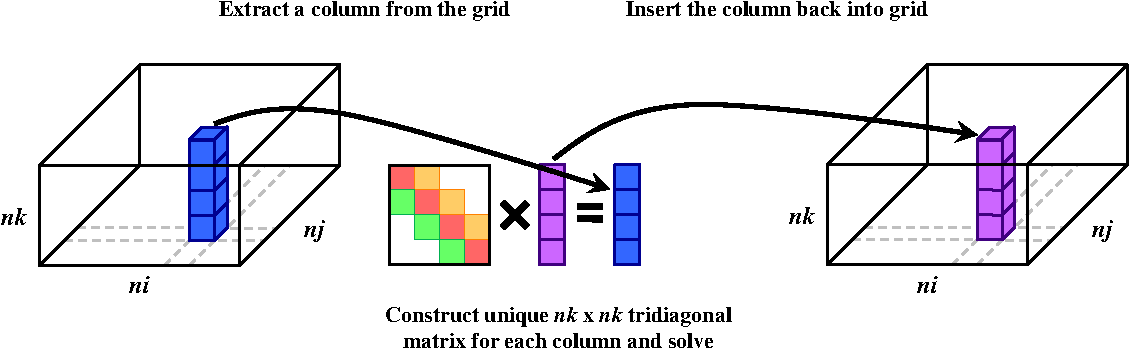
\includegraphics[width=0.95\textwidth]{figures/batching/independent_solve_diagram.pdf}
\end{figure*}

\begin{figure*}[!bth]
  \centering
  \caption{\small
    \textbf{Simultaneous Solve Strategy:} A tile of vertical columns, each 
      containing \(nk\) elements, is extracted from a \(ni \times nj \times nk\)
      3D Cartesian grid.
    All the columns in the tile are solved simultaneously, interleaving 
      the computation of individual solves.
    This approach exposes task parallelism, exhibits good data locality and
      enables vectorization in one of the horizontal dimensions (\(i\)).
    SSTA uses this strategy.
  }
  \label{fig:impl:batching:sim_strat}
  %\vspace{1em}
  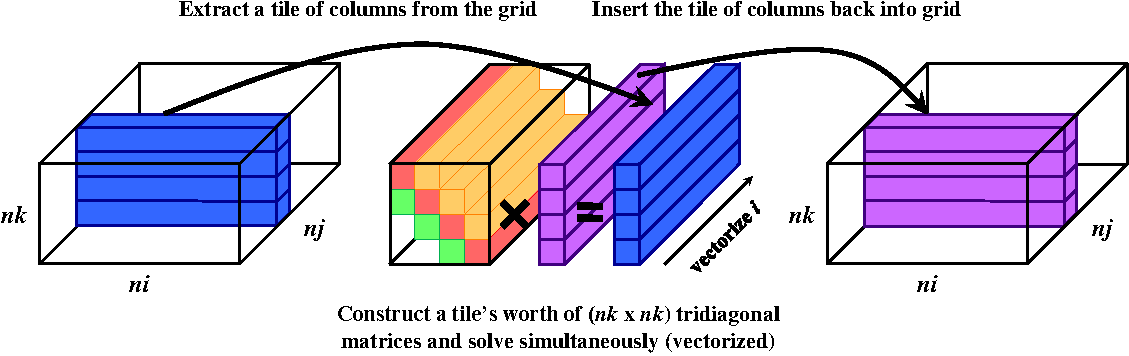
\includegraphics[width=0.95\textwidth]{figures/batching/simultaneous_solve_diagram.pdf}
\end{figure*}

We can use a simplified form of Gaussian elimination that does not require
  pivoting, known as the Thomas algorithm or the tridiagonal matrix algorithm
%  (TDMA)~\cite{elem_numerical_analysis_conte,numerical_math_quarteroni}, to
  (TDMA)~\cite{elem_numerical_analysis_conte}, to
  solve the type of system described in the previous section.
The Thomas algorithm takes advantage of sparsity to be \(O(nk)\) in time, 
  and can be extended to banded matrices and LU factorizations.
It is also a significant improvement over dense Gaussian elimination,
  which is \(O(nk^3)\) in time. 
We use a formulation of the Thomas algorithm which does not require any storage
  for temporary values, but overwrites the \(b\) vector and solves for
  \(u^{s+1}\) in place, overwriting \(u^{s}\).

The Thomas algorithm consists of two passes.  First, a forward pass is
  performed to eliminate the \(a_i\) elements:
\begin{lstlisting}
for (auto k = 1; k < nk; ++k) {
  auto const m = a[k] / b[k - 1];
  b[k] -= m * c[k - 1];
  u[k] -= m * u[k - 1];
} 
\end{lstlisting}
Then, an abbreviated form of back substitution is performed to obtain the
  solution:
\begin{lstlisting}
u[nk - 1] = u[nk - 1] / b[nk - 1];

for (auto k = nk - 2; k >= 0; --k) 
  u[k] = (u[k] - c[k] * u[k + 1]) / b[k];
\end{lstlisting}

The Thomas algorithm has very low algorithmic intensity (AI)~\cite{roofline}.
During the course of our work, we developed a \textbf{theoretical peak
  performance model} for the Thomas algorithm.

First, we count the number of FLOPs performed.
We will consider multiplications, additions and division operations as FLOPs.
Each iteration of the forward elimination loop contains 1 division, 2
  multiplications and 2 subtractions.
This gives us a total of either \(3(nk-1)\) FLOPs on fused-multiply-add (FMA)
  architectures~\cite{intel_sw_dev_manual_2c} or 
  \(5(nk-1)\) FLOPs on non-FMA architectures.
Next, the pre-substitution operation (the assignment to \lstinline{u[nk - 1]}
  in the above snippet) performs a single division.
Finally, the back substitution loop performs 1 multiplication, 1
  subtraction and 1 division, adding either \(2(nk-1)\) FLOPs (FMA architectures)
  or \(3(nk-1)\) FLOPs (non-FMA architectures).
In total, this gives us either \(5nk-4\) FLOPs (FMA) or \(8nk-7\) FLOPs
  (non-FMA) for the entire Thomas algorithm.

Our data movement model for the Thomas algorithm assumes that we will achieve
  optimal performance when data is cached between the forward elimination and
  back substitution loop.
That is, we assume that accesses to \(a\), \(b\), \(c\) and \(u\) will
  \textbf{not} go to main memory in the back substitution loop because the
  arrays still reside in the cache hierarchy from the forward elimination loop
  accesses.

The Thomas algorithm accesses four arrays, reading from all of them (\(a\),
  \(b\), \(c\) and \(u\)) and writing to two of them (\(b\) and \(u\)).
\(b\) and \(u\) have extent \(nk\), so we store \(2nk\) elements.
\(a\) and \(c\) have extent \(nk-1\), so we load \(2(nk-1)+2nk\) elements.
In total, \(6nk-2\) elements are moved.
Assuming double precision, \(48nk-16\) bytes are moved to and from main memory
  during execution of the Thomas algorithm.

This gives us a FLOPs/byte ratio of \((5nk-4)/(48nk-16)\) (FMA) or
  \((8nk-7)/(48nk-16)\) (non-FMA).
The lower bound for the Thomas algorithm's arithmetic intensity is \(1/32\)
  FLOPs/byte when \(nk=1\). 
The upper bound is \(5/48\) FLOPS/byte (FMA) or \(1/6\) FLOPs/byte (non-FMA) as
  \(nk\) approaches infinity.
Based on this analysis, we can conclude that the Thomas algorithm is
  \textbf{memory-bandwidth bound}.
Thus, we use effective bandwidth, not FLOPs, as our performance metric.

We verified our analytic model by measuring hardware performance counters which
  track memory traffic with the Intel VTune Amplifier XE
  profiler~\cite{intel_vtune_amplifier}.
We found that memory bandwidth measured via hardware counters generally agreed
  with our model. 

\subsection{Batching and Vectorization}
\label{sec:impl:batching_and_parallelism}

In the applications described in \S\ref{sec:intro} we need to apply the
  Thomas algorithm to each vertical column in a \(ni \times nj \times nk\)
  3D Cartesian grid, where \(i\) and \(j\) are \textbf{horizontal dimensions}
  and \(k\) is the \textbf{vertical dimension}.
These computations are known as the \textbf{vertical solves}.
Since each vertical solve is independent of the others, this is an
  embarrassingly parallel problem.
The matrix coefficients for each column depend on the problem state, so a
  unique matrix for each column needs to be constructed before each solve.
There are two different approaches to computing these batch solves.

The most straightforward approach is \textbf{solve} each column
  \textbf{independently} (the \textbf{independent solve strategy}; Figure
  \ref{fig:impl:batching:ind_strat}).
An \(nk \times nk\) tridiagonal matrix is constructed for each column, and then
  the Thomas algorithm is used to solve the system formed by the matrix and the
  vertical column.
Because the vertical solves are independent, they can be executed concurrently
  via task-level parallelism.
Vectorization of the \(nk\) loop is not possible as each iteration of the loops
  in the Thomas algorithm is dependent on the previous iteration (e.g.
  loop-carried dependency)~\cite{pipelined_thomas_algorithm}.

The other approach is to \textbf{simultaneously solve} multiple columns (the
  \textbf{simultaneous solve strategy}; Figure
  \ref{fig:impl:batching:sim_strat}).
A block \(nk \times nk\) tridiagonal matrix is constructed for the whole grid;
  each block contained within the matrix is an \(ni \times nj\) horizontal plane
  (e.g. the block matrix is a 4D space).
To perform the vertical solves, we view the entire 3D Cartesian grid as an
  \(nk\) block vector of \(ni \times nj\) planes and apply it to the block
  matrix.
Each step of the algorithm is applied across an entire plane.
The forward sweep becomes:
\begin{lstlisting}
for (auto k = 1; k < nk; ++k)
 for (auto j = 0; j < nj; ++j)
  for (auto i = 0; i < ni; ++i) {
    auto const m = a[i][j][k]
                 / b[i][j][k - 1];
    b[i][j][k] -= m * c[i][j][k - 1];
    u[i][j][k] -= m * u[i][j][k - 1];
  } 
\end{lstlisting}
This approach facilities both task-level parallelism and vectorization.
The grid and block matrix can be tiled into smaller subgrids, and the Thomas
  algorithm can be applied to each subgrid independently.
Each step of the Thomas algorithm can be vectorized across the \(ni \times nj\)
  horizontal plane that it is operating on: e.g. the \(i\) loop in the
  above snippet can be vectorized.

Our MKL baseline solver uses the independent solve approach, while SSTA uses
  the simultaneous solve strategy.
The vector parallelism exposed by the simultaneous approach offers a major
  benefit over the independent approach.
It is necessary to vectorize even for a memory-bandwidth bound problem like the
  Thomas algorithm, as peak memory bandwidth cannot be achieved without
  exploiting wider vector loads and stores.
Such vectorization is not possible with most of the loops in the independent
  approach due to data dependencies between iterations of the Thomas
  algorithm~\cite{pipelined_thomas_algorithm}.
Even if it was possible to vectorize in the vertical dimension \(k\), it would
  still be undesirable to do so.
The extent of the vertical dimension tends to be very small in the applications
  we are concerned with (\(O(30-100)\)), so loop and vectorization overheads
  would be hard to amortize.

\subsection{Data Layout}
\label{sec:impl:data_layout}

The data layout of the Cartesian grid has a huge impact on the performance
  of our solver.
Throughout the course of our research, our understanding of the impact of
  different data layouts has evolved substantially.
We have investigated three different schemes: \(kji\), \(ijk\) and \(kji\)
  (Table~\ref{tab:impl:layout:types}).

\begin{figure*}[!bth]
  \centering
  \caption{\small
    \textbf{Example of Different Layouts and Tiling Schemes:}
      The SSTA solver supports four layout and tiling scheme combinations.
      The figures below show how the different combinatons would partition an
        \(a \times a \times b\) grid into four tiles each containing
        \((a^2/4)(b)\) elements (one tile is shown).
      With the tile-\(ij\) scheme we get \(a/2 \times a/2 \times b\) tiles,
        and with the tile-\(i\) scheme we get \(a \times a/4 \times b\) tiles.
      Different colors indicate different contiguous regions within the tile.
      Regions with similar colors have greater locality with each other. 
  }
  \label{fig:impl:tiling_schemes}
  %\vspace{1em}
  \begin{minipage}{0.49\textwidth}
    \centering
    \subfloat[
      \textbf{\(ijk\)-Layout with the Tile-\(ij\) Scheme:}
      \((a/2)(b)\) contiguous \(i\)-rows each containing \(a/2\) elements.
      This layout and tiling combination exhibits the worst contiguity out of the
        four different options.
    ]{        
      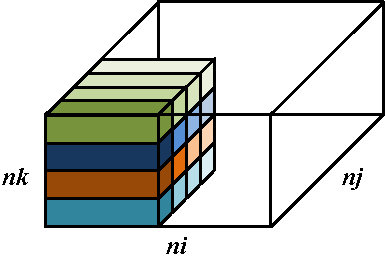
\includegraphics[width=0.70\columnwidth]{figures/tiling/ijk_layout_tile_ij_scheme_diagram.pdf}
      \label{fig:impl:tiling:ijk_tile_ij_scheme}
    }
  \end{minipage}
  \begin{minipage}{0.49\textwidth}
    \centering
    \subfloat[
      \textbf{\(ijk\)-Layout with the Tile-\(j\) Scheme:}
      \(b\) contiguous \(ij\)-planes, each containing \(a^2/4\) elements.
      This layout and tiling combination exhibits the best contiguity for the 
        \(ijk\)-layout.
    ]{
      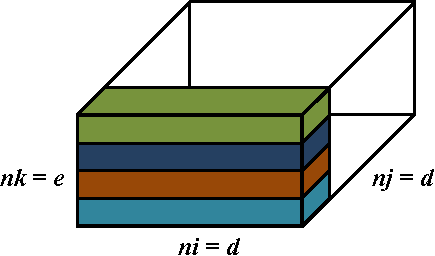
\includegraphics[width=0.70\columnwidth]{figures/tiling/ijk_layout_tile_j_scheme_diagram.pdf}
      \label{fig:impl:tiling:ijk_tile_j_scheme}
    }
  \end{minipage}
  \hspace{0em}
  \begin{minipage}{0.49\textwidth}
    \centering
    \subfloat[
      \textbf{\(ikj\)-Layout with the Tile-\(ij\) Scheme:}
      \((a/2)(b)\) contiguous \(i\)-rows, each containing \(a/2\) elements.
      This layout and tiling combination exhibits the worst contiguity out of the
        four different options.
    ]{        
      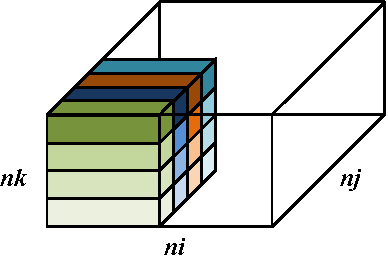
\includegraphics[width=0.70\columnwidth]{figures/tiling/ikj_layout_tile_ij_scheme_diagram.pdf}
      \label{fig:impl:tiling:ikj_tile_ij_scheme}
    }
  \end{minipage}
  \begin{minipage}{0.49\textwidth}
    \centering
    \subfloat[
      \textbf{\(ikj\)-Layout with the Tile-\(j\) Scheme:}
      One contiguous region containing \((a^2/4)(b)\) elements.
      This layout and tiling combination exhibits the greatest contiguity out of
        the four different options, and provides the best performance on
        Knight's Landing.
    ]{
      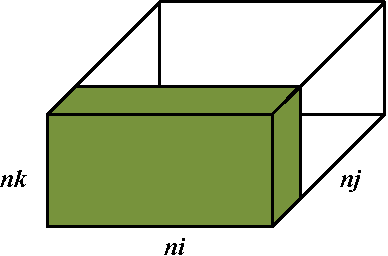
\includegraphics[width=0.70\columnwidth]{figures/tiling/ikj_layout_tile_j_scheme_diagram.pdf}
      \label{fig:impl:tiling:ikj_tile_j_scheme}
    }
  \end{minipage}
\end{figure*}

\begin{table}[h]
\centering
% NOTE: kji AKA column-major, Fortran, left
% NOTE: ijk AKA row-major, C++, right
\caption{\textbf{Data Layouts for the 3D Cartesian Grid}}
\begin{tabular}[t]{|l|rr|r|} \hline
%%%%%%%%%%%%%%%%%%%%%%%%%%%%%%%%%%%%%%%%%%%%%%%%%%%%%%%%%%%%%%%%%%%%%%%%%%%%%%%
  \multicolumn{1}{|c|}{\multirow{2}{*}{\textbf{Name}}}
& \multicolumn{1}{ c }{\textbf{\(i\)-stride}}
& \multicolumn{1}{ c|}{\textbf{\(j\)-stride}}
& \multicolumn{1}{ c|}{\textbf{\(k\)-stride}} \\
%%%%%%%%%%%%%%%%%%%%%%%%%%%%%%%%%%%%%%%%%%%%%%%%%%%%%%%%%%%%%%%%%%%%%%%%%%%%%%%

& \multicolumn{2}{c|}{\textbf{(Horizontal)}}

& \multicolumn{1}{c|}{\textbf{(Vertical)}}   \\ \thickhline
%%%%%%%%%%%%%%%%%%%%%%%%%%%%%%%%%%%%%%%%%%%%%%%%%%%%%%%%%%%%%%%%%%%%%%%%%%%%%%%
  \(ijk\), Column-Major
& \multicolumn{1}{r|}{\(1\)}
& \multicolumn{1}{r|}{\(ni\)}
& \((ni)(nj)\)                              \\ \hline
%%%%%%%%%%%%%%%%%%%%%%%%%%%%%%%%%%%%%%%%%%%%%%%%%%%%%%%%%%%%%%%%%%%%%%%%%%%%%%%
  \(kji\), Row-Major
& \multicolumn{1}{r|}{\((nj)(nk)\)}
& \multicolumn{1}{r|}{\(nk\)}
& \(1\)                                     \\ \hline
%%%%%%%%%%%%%%%%%%%%%%%%%%%%%%%%%%%%%%%%%%%%%%%%%%%%%%%%%%%%%%%%%%%%%%%%%%%%%%%
  \(ikj\)
& \multicolumn{1}{r|}{\(1\)}
& \multicolumn{1}{r|}{\((ni)(nz)\)}
& \(ni\)                                    \\ \hline
%%%%%%%%%%%%%%%%%%%%%%%%%%%%%%%%%%%%%%%%%%%%%%%%%%%%%%%%%%%%%%%%%%%%%%%%%%%%%%%
\end{tabular}
\label{tab:impl:layout:types}
\end{table}

The production code that our MKL baseline solver is derived from uses the
  \(ijk\)-layout.
The vertical columns that we need to pass in to MKL as the right-hand side
  (\(u\)) are non-contiguous, as the vertical dimension \(k\) is the dimension
  with greatest stride.
Currently, the production codebase allocates a temporary gather buffer, copies
  data from the grid into the buffer, calls the LAPACK solver, and then copies
  the result from the buffer back to the grid.

We have found the \(kji\)-layout to be optimal for our MKL baseline solver.
With the \(kji\)-layout, we have contiguous vertical columns which can be
  passed to MKL without temporary allocations or unnecessary copies.
We observed a noticeable performance increase from this optimization with very
  little source code change, although we have not studied the impact of this
  layout change on other components in more complex, multi-kernel applications.

Our SSTA solver uses either the \(ijk\)- or \(ikj\)-layout.
SSTA vectorizes in one of the horizontal directions, so it is
  desirable to use layouts where the horizontal dimension that we are
  vectorizing (\(i\)) is the unit stride dimension, avoiding strided vector loads.
The \(ikj\)-layout arose as an optimization to combat data locality and
  prefetching issues which hindered performance on the Intel Xeon Phi Knight's
  Landing architecture, and is described in greater detail in the following
  section and in \S\ref{sec:results}.

\subsection{Tiling}
\label{sec:impl:tiling}

To ensure good CPU cache utilization, it is often necessary to break a larger
  grid into smaller \textbf{tiles} which better amortize nested loop overheads, expose
  greater data locality and keep data resident in a particular level of the
  cache hierarchy~\cite{cache_blocking}.
This technique is also known as \textbf{cache blocking}.
Additionally, partitioning a grid with dimensions known only at application
  initialization into fixed size tiles can provide some of the performance
  benefits of compile-time-fixed dimensions (via compiler optimizations) with
  the flexibility of a dynamically sized problem~\cite{kokkos}.
Tiling also provides a useful abstraction for parallel work distribution, as
  each tile can be computed independent of other tiles and has no overlapping
  data accesses.
Tiling is particularly important for memory-bandwidth bound computations like
  tridiagonal matrix solves.

The production code which our MKL baseline solver is derived from is not task
  parallelized or explicitly tiled.
Since each column is solved independently, there is little opportunity to improve
  locality and reuse via tiling (shown in \S\ref{sec:results}).
Conceptually, since each column is solved independently in the production code,
  it is \textbf{effectively} tiled, albeit with a very small tile size (a single
  column, e.g. \(O(30-100)\)).
Our MKL baseline solver is tiled solely to facilitate task parallelization.

On the other hand, tiling is very fundamental to our SSTA solver.
Our performance model (\S\ref{sec:impl:thomas_algorithm})
  is based on caching assumptions which we rely on tiling to enforce.
In particular, we assume that all four arrays (\(a\), \(b\), \(c\) and \(u\))
  remain in the cache hierarchy in between the loops. 
If any of these four arrays need to be reloaded from main memory in between the
  forward elimination and back substitution loops, the amount of main memory data
  movement is significantly increased and the algorithmic intensity of the
  algorithm decreases dramatically.
While our untiled SSTA results outperform the MKL baseline results (Figure
  \ref{fig:results:percent_stream_bw}), they were well below the manufacturer-specified
  bandwidth and STREAM Triad effective bandwidth.
On the platforms covered in this paper, we typically aim to fit within the L2
  cache.

It is important to note the distinction between \textbf{per-array tile size}
  (e.g. the tile size for one of the four arrays) and the
  \textbf{total tile size} (e.g. the sum of the per-array tile sizes).
The total tile size is the amount of data we need to remain in cache between
  the forward elimination and back substitution loops.
Unless stated otherwise, when we refer to ``tile size'' we mean
  total tile size.

Due to the loop-carried dependencies in the Thomas algorithm and the small
  extent of \(nk\), we could not tile the vertical dimension. So, we explored two
  tiling schemes which partition the horizontal \(ij\)-plane.

The \textbf{tile-\(ij\)} scheme partitions both the \(i\) and \(j\) dimensions,
  yielding tiles with arbitrary horizontal shape. 
The \textbf{tile-\(j\)} scheme partitions only the \(j\) dimension, producing
  tiles containing contiguous \(i\)-rows.
There is a trade-off between these two schemes, with the tile-\(ij\) scheme
  offering greater flexibility in tile size and the tile-\(j\) scheme offering
  greater contiguity. 

For example, suppose we partition an \(ijk\)-layout grid into four tiles each
  containing \((a^2/4)(b)\) elements, with the tile-\(ij\) scheme producing
  \(a/2 \times a/2 \times b\) tiles
  (Figure~\ref{fig:impl:tiling:ijk_tile_ij_scheme})
  and the tile-\(i\) scheme producing
  \(a \times a/4 \times b\) tiles
  (Figure~\ref{fig:impl:tiling:ijk_tile_j_scheme}).
For the tile-\(ij\) scheme, tiles contain \((a/2)(b)\) contiguous
  \(i\)-rows of only \(a/2\) elements each.
For the tile-\(j\) scheme, tiles contain \(b\) contiguous \(ij\)-planes of
  \(a^2/4\) elements each.

While the tile-\(j\) scheme offers greater contiguity than the
  tile-\(ij\) in this example, the tile-\(j\) tiles are not a single contiguous
  memory region with the \(ijk\)-layout.
The only way to obtain completely contiguous tiles in the \(ijk\)-layout would
  be to tile the dimension with the greatest stride (\(k\)), which is not an
  option as we never partition the vertical dimension.

This limitation led us to the \(ikj\)-layout for the SSTA solver (see
  \S\ref{sec:results}).
With this layout, the direction of vectorization (\(i\)) is still the unit stride
  dimension, avoiding strided loads and assisting hardware prefetching.
Additionally, the tile-\(j\) tiles are completely contiguous regions of memory,
  decreasing translation-lookaside buffer (TLB) pressure, increasing locality for
  caching and further assisting hardware prefetching.

Consider switching to the \(ikj\)-layout in the previous example.
The tile-\(ij\) tiles would be the same as before: \(a/2 \times a/2 \times b\)
  tiles consisting of \((a/2)(b)\) contiguous \(i\)-rows of only \(a/2\)
  elements each (Figure~\ref{fig:impl:tiling:ikj_tile_ij_scheme}).
The tile-\(j\) tiles would be one contiguous region containing all
  \((a^2/4)(b)\) elements
  (Figure~\ref{fig:impl:tiling:ikj_tile_j_scheme}).

The only notable downside to the tile-\(j\) scheme is the loss of
  flexibility in tile sizes.
The smallest tile size for the tile-\(j\) scheme is a \(a \times 1 \times b\)
  tile (an \(ik\) plane), while the smallest tile size for the
  tile-\(ij\) scheme is a \(1 \times 1 \times b\) tile (a single column).
We have not found this restriction to be overly restrictive.

We present results with the tile-\(j\) scheme and both the \(ijk\)- and
  \(ikj\)-layout in this paper.

%%%%%%%%%%%%%%%%%%%%%%%%%%%%%%%%%%%%%%%%%%%%%%%%%%%%%%%%%%%%%%%%%%%%%%%%%%%%%%%
\section{Experimental Setup}
\label{sec:setup}
We developed the Tridiagonal Solve Benchmarks (TSB) suite during the course of
  our research~\cite{tsb_git}.
The TSB suite is freely available on Github under the Boost Software License,
  version 1.0.
%  version 1.0~\cite{boost_license}.
%Git tag \lstinline{ssta_paper_09_2016} contains the source code used for the
%  experiments in this paper.
The benchmark suite has three major components: a multi-dimensional array
  abstraction, generic solver components and a test harness.

\subsection{Test Problem}
\label{sec:setup:test_problem}

The benchmarks in the TSB suite solve a matrix in each vertical column derived
  from a simple implicit Backward Time, Centered Space (BTCS) finite difference
  stencil with Dirichlet boundary conditions every time step.
The diagonally-dominant tridiagonal matrix takes the following form,
  where \(D\) is a dimensionless diffusion coefficient (\(D > 0\)),
  \(\Delta \, t\) is the time step size, \(\Delta \, k\) is the vertical grid
  spacing and \(r=D \, \Delta \, t / \Delta \, k < 1/2\):
\begin{align*}
A = 
\begin{bmatrix}
1   & 0      &     &        & 0  \\
-r  & 1 - 2r & -r  &        &    \\
    & ...    & ... & ...    &    \\
    &        & -r  & 1 - 2r & -r \\
0   &        &     & 0      & 1
\end{bmatrix}  
\end{align*}
An identical form of the problem is initialized in every vertical column of the
  grid.

\subsection{Hardware Platforms}
\label{sec:setup:hardware_platforms}

The TSB suite currently targets x86-64 microarchitectures with SIMD vector units
  running POSIX-compliant operating systems.
The results presented in this paper were collected from both Intel Xeon and
  Xeon Phi systems.

%Our two Intel Xeon platforms, Edison~\cite{nersc_edison_config} and Cori Phase
%  1~\cite{nersc_cori_p1_config}, are homogeneous Cray supercomputers,
%  consisting of traditional dual-socket x86-64 nodes.
Our two Intel Xeon platforms, Edison and Cori Phase 1, are homogeneous Cray
  supercomputers, consisting of traditional dual-socket x86-64
  nodes~\cite{nersc_systems}.
Edison features Intel Xeon E5-2695 v2 Ivy Bridge
  (IVB) processors~\cite{intel_ark_xeon_e5_2695_v2}, and Cori Phase 1 has Intel
  Xeon E5-2698 v3 Haswell (HSW) processors~\cite{intel_ark_xeon_e5_2698_v3}.
In general, the two Xeon platforms have a very similar performance profile for
  our application.
Commensurate with MPI parallelization for distributed memory, in all experiments
  we restricted ourselves to a single NUMA nodel
%As cluster-on-die (COD) is not enabled on our Xeon Phi platform, one NUMA node
%  corresponds to a single socket on each of our test systems.

Our Xeon Phi testbed, which features Intel Xeon Phi 7210 Knight's Landing
  (KNL) processors~\cite{intel_ark_xeon_phi_7210}, is notably different from
  the two Xeon systems.
Knight's Landing is a many-core design with a 2D mesh of \textbf{lightweight}
  cores optimized for throughput and explicit parallelism at the expense of
  increased latency and reduced complexity in other areas (branch prediction,
  out-of-order execution facilities, pipeline depth, etc).
The KNL microarchitecture has a number of novel features including on-package
  high-bandwidth MCDRAM, 4 hyper-threads per core and dual 512-bit
  AVX512 vector units.~\cite{roofline_knl,knl_sodani}

Knight's Landing processors can be configured for different Non-Uniform Memory
  Access (NUMA) topologies.
Additionally, the MCDRAM can be configured as programmable memory, a
  direct-mapped last-level cache or a combination of the
  two~\cite{knl_sodani}.
For all experiments in this paper, we used a
  \lstinline{quadcache}~\cite{roofline_knl} configuration, where all processing
  units are in a single NUMA domain and all 16GB of MCDRAM are used as a cache.

\subsection{Toolchain}
\label{sec:setup:toolchain}

TSB is written in ISO C++14~\cite{cxx14_spec} and has no external software
  dependencies.
The code contains no vector intrinsics or vector assembly.
We rely entirely on the compiler vectorization engine for performant vector
  code generation, utilizing compiler directives to guide parallelization and
  vectorization, and indicate alignment, loop trip count and aliasing
  assumptions.
%Avoiding vector intrinsics and hand-written assembly makes TSB performance
%  portable between different x86-64 vector instruction sets (SSE, AVX, AVX2,
%  AVX512) and simplifies porting to other architectures (such as GPGPUs).
%We have also found it leads to better code generation by giving the compiler
%  the freedom to select the correct instructions and perform optimizations which
%  we have found to be inhibited by explicit vector intrinsics, such as
%  post-vectorization loop unrolling.

SSTA is task-parallelized using OpenMP \lstinline{#pragma}s~\cite{openmp_spec}.
Since the problem is embarrassingly parallel in the horizontal dimensions, it
  is easy to statically load balance (dimension extents and tile sizes
  permitting).
%The Portable Hardware Locality (hwloc) topology
%  framework~\cite{hwloc} is used to pin OpenMP threads to hardware execution
%  resources.

The Intel C++ Compiler~\cite{intel_cpp_compiler} was used to compile the TSB
  suite for all of the results presented in this paper.
We used the 2017 Beta Update 2 version (\lstinline{17.0.0 20160517}).
We also used the Intel VTune Amplifier XE general-purpose
  profiler~\cite{intel_vtune_amplifier} during our research.
%We also used the Intel VTune Amplifier XE general-purpose
%  profiler~\cite{intel_vtune_amplifier} and the Intel Advisor XE vectorization
%  and threading profiler~\cite{intel_advisor} during our research.
%Both tools are sampling profilers which can gather and analyze data from
%  hardware-based performance monitoring facilities.

\subsection{Statistical Considerations}
\label{sec:setup:stats}

\textbf{Effective bandwidth} is our primary performance metric.
We define effective bandwidth as \textbf{effective data movement} \(/\)
  \textbf{solver execution time}.

We use the theoretical peak performance model for data movement in the Thomas
  algorithm defined in \S\ref{sec:impl:thomas_algorithm} to estimate
  effective data movement.
To measure solver execution time, we record and average the wall-clock
  execution time of each timestep. 
We include OpenMP parallelization in our measurements, e.g. we time the
  \lstinline{#pragma omp for} loop instead of measuring the duration of each
  tile-iteration individually.
Thus, parallel overheads are included in our recorded execution times.
%Time is measured using \lstinline{std::chrono::steady_clock}, which uses a
%  system clock that is monotonically
%  increasing~\cite{cppreference_chrono_steady_clock}.
%On the three platforms we ran on, \lstinline{std::chrono::steady_clock} has
%  nanosecond resolution.

We performed each individual experiment a statistically significant number of 
  times on different nodes of our test systems.
Sample sizes varied between experiments and platforms, but were usually between
  100 to 200 independent executions per data point.
We estimated variance between \textbf{different
  executions} of the benchmark with identical parameters by computing sample
  standard deviation.
All measurements presented are \textbf{95\% confidence intervals} (depicted
  visually with bars on all graphs) constructed from the mean and sample standard
  deviation of the dataset.

We used STREAM~\cite{stream} Triad results as an reference for peak effective
  bandwidth.
We measured STREAM Triad bandwidth between 49.74 GB/s and 49.86 GB/s on our Ivy
  Bridge system, between 60.36 GB/s and 60.44 GB/s on our Haswell system and
  between 418.2 GB/s and 419.6 GB/s on our Knight's Landing system.

We believe there are two potential sources of non-trivial \textbf{systemic
  observational error} in our results.
First, mistakes in our analytic performance model for data movement could
  potentially skew our data.
We mitigated this by verifying the model with hardware-based
  profilers (Intel VTune Amplifier XE~\cite{intel_vtune_amplifier}), and we are
  confident in its validity.
Second, variance in the execution time of \textbf{individual timesteps} is not
  accounted for.
We currently average the execution time of all timesteps
  within a single execution of a benchmark, but do not compute and record
  sample standard deviation as a variance estimation \textbf{within} the solver.
Removing this source of systemic error would be straightforward, but
  would require extending our postprocessing framework to compute running 
  sample standard deviations~\cite{benchmarking_cxx_code} which we have not
  yet implemented.
%Sources of \textbf{random observational error} include work starvation and
%  varying performance of the memory subsystem due to system variance and OS
%  noise.

%%%%%%%%%%%%%%%%%%%%%%%%%%%%%%%%%%%%%%%%%%%%%%%%%%%%%%%%%%%%%%%%%%%%%%%%%%%%%%%
\section{Results}
\label{sec:results}

\begin{figure*}[!bth]
  \centering
  \caption{\small
    \textbf{SSTA Effective Bandwidth vs. Total Tile Size:}
    The results of a parameter sweep on our two Intel Xeon platforms
      demonstrating the effect of total tile size on the performance of the
      SSTA solver is shown below (MKL baseline and STREAM Triad results shown as
      lower- and upper-bounds).
%    For the \(ijk\)-layout, the optimal tile size, 256KB, is too large to fit
%      within the L2 cache.
%    Smaller tile sizes perform poorly for this layout because data contiguity
%      decreases with the tile size, incurring TLB and hardware prefetching
%      penalties.
%    The optimal tile size for the \(ikj\)-layout is 32KB, which fits in the L2. 
    The \(ikj\)-layout, which exhibits better contiguity and memory access
      patterns, performs better at smaller tile sizes, although the best
      \(ikj\)-layout result does not outperform the best \(ijk\)-layout result
      on these platforms.
    Performance degrades for tile sizes which exceed L3 capacity per core.
    Both SSTA variants substantially outperform the MKL baseline results and 
      reach \textapprox 90\% of STREAM Triad effective bandwidth with optimal 
      tile sizes.
    Results are shown with 95\% confidence.
  }
  \label{fig:results:bw_vs_tile_size_xeon}
  %\vspace{1em}
  \begin{minipage}{0.49\textwidth}
    \subfloat[
      \textbf{Ivy Bridge}
    ]{        
      \includegraphics[width=0.99\columnwidth]{figures/results/effective_bandwidth_vs_total_tile_size_edison_ivb_e5_2695_v2_1socket_graph.pdf}
      \label{fig:results:bw_vs_tile_size_ivb}
    }
  \end{minipage}
  \begin{minipage}{0.49\textwidth}
    \subfloat[
      \textbf{Haswell}
    ]{
      \includegraphics[width=0.99\columnwidth]{figures/results/effective_bandwidth_vs_total_tile_size_cori_hsw_e5_2698_v3_1socket_graph.pdf}
      \label{fig:results:bw_vs_tile_size_hsw}
    }
  \end{minipage}
\end{figure*}

\begin{figure}[!h]
  \centering
  \caption{\small
    \textbf{SSTA Effective Bandwidth vs. Total Tile Size (Knight's Landing):}
    Shown below are the results of a parameter sweep on our Intel Xeon Phi
      Knight's Landing platform showing the effect of data layout and total
      tile size on the performance of the SSTA solver.
    MKL baseline (lower-bound) and STREAM Triad (upper-bound) results are shown
      for reference.
%    The optimal tile size for the \(ijk\)-layout is 128KB, and the optimal
%      tile size for the \(ikj\)-layout is 32KB.
%    Both will fit in the L2 cache.
    \(ijk\)-layout performance is hampered by poor data contiguity which incurs
      expensive TLB and hardware prefetching penalties on Knight's Landing.
    This effect is amplified at smaller tile sizes.
    The best \(ikj\)-layout result has between 91 GB/s and 109 GB/s higher
      effective bandwidth than the best \(ijk\)-layout result, and reaches
      between 88\% and 92\% of STREAM Triad performance.
%    The \(ikj\)-layout is a \(12x\) speedup and the \(ijk\)-layout is a
%      \(9x\) speedup over the MKL solver.
    Results are shown with 95\% confidence.
  }
  \label{fig:results:bw_vs_tile_size_knl}
  \includegraphics[width=0.95\columnwidth]{figures/results/effective_bandwidth_vs_total_tile_size_carl_knl_7210_1socket_graph.pdf}
\end{figure}

\begin{figure}[!h]
  \centering
  \caption{\small
    \textbf{Percentage of STREAM Triad Effective Bandwidth Attained by SSTA:}
    Across all three microarchitectures, the SSTA solver with an optimal tile
      size improves performance substantially over the MKL baseline, and
      achieves \textapprox 90\% of STREAM Triad effective bandwidth.
    Although untiled SSTA results beat the MKL solver, tiling contributes
      significantly to overall performance: between 35.9\% and 36.1\% on 
      Ivy Bridge, 34.22\% and 35.38\% on Haswell and 24\% and 26\% on 
      Knight's Landing.
    Between 21\% and 25\% of STREAM performance attained is attributed to the
      switch to the \(ikj\)-layout on Knight's Landing. 
    Results are shown with 95\% confidence.
  }
  \label{fig:results:percent_stream_bw}
  \includegraphics[width=0.95\columnwidth]{figures/results/percentage_of_stream_bw_attained_histogram.pdf}
\end{figure}

% Hypothesis 1.1: SSTA can outperform legacy solver
% Hypothesis 1.2: SSTA can efficiently utilize memory bandwidth 
% Prediction 1.1 and Prediction 1.2 follow naturally 
We developed SSTA to replace the underperforming MKL-based vertical column
  solver in our production climate application because we believed that a new
  algorithm which solves multiple vertical columns simultaneously would
  efficiently utilize available memory bandwidth and significantly outperform the
  legacy solver by exhibiting performant data movement patterns and facilitating
  vectorization.

% Hypothesis 2: SSTA will be highly sensitive to data layout changes and total
% tile size and will achieve optimal performance for a particular tile size
% that balances reuse/locality/amortization.
We also theorized that such a solver would be highly sensitive to
  \textbf{data layout changes} and
  \textbf{total tile size} (\S\ref{sec:impl:tiling}).
Parallel application performance is often driven by parameters such as 
  tile size, which control the amount of work in each parallel task.
In memory-bandwidth bound applications, data layout and tiling can be
  especially important as they not only influence the amount of task- and
  vector-parallelism exposed but also the working set size and degree of cached
  data reuse in each individual task.
We anticipated that we would need to study the effect of different data layouts
  and tile sizes in order to understand the performance of our new solver.
The first step was to determine the \textbf{optimal total tile size} for the 
  different solver variants in the TSB suite.

We conducted a parameter sweep of total tile size on our Xeon and Xeon Phi 
  platforms.
We predicted that we would see the following: 
\begin{itemize}
% Prediction 2.1: The MKL solver doesn't care about tile size, excluding
% SLOW effects.
\item The MKL baseline solver would be very insensitive to total tile size,
  excluding extremely small (high overhead) and extremely large (insufficient
  parallelism) sizes since it solves each column independently and thus cannot
  exploit vector operations and data locality like the SSTA solver does.
% Prediction 2.2: Total tile sizes which fit in the L1D will be too small to be
% feasible.
\item Total tile sizes small enough to fit into the L1D cache would not be
  feasible because the overheads of loop constructs and
  parallelization/vectorization setup would be too great relative to the
  execution time of useful work per inner-loop iteration.
These tile sizes would either require vertical extents below the sizes 
  we are interested in (\(nk < 16\)) or horizontal
  dimensions too small to vectorize efficiently (\(ni < 16\)).
% Prediction 2.3: Optimal total tile size will be in between L1D capacity and
% L2 capacity.
\item The optimal total tile size would fit into the L2 cache (but not the L1D
  cache), since it is the fastest cache which has the capacity to contain a
  feasible tile size.
% Prediction 2.4: Performance drops as total tile size crosses cache capacity
% boundaries, excluding L1D.
\item Excluding the L1D, as we move from a tile size which fits into the
  capacity of a particular cache to a tile size which does not, we should see a
  drop in effective bandwidth.
On the Xeon platforms, the boundaries are L2 \(\rightarrow\) L3 and L3
  \(\rightarrow\) DRAM (main memory).
On Knight's Landing, the boundaries are L2 \(\rightarrow\) MCDRAM and MCDRAM
  \(\rightarrow\) DRAM (main memory).
\end{itemize}
Note that when a total tile size is equal to a particular cache capacity, we
  claim that it will \textbf{not} entirely fit into that cache, since it is not
  reasonable to assume that our arrays will be able to consume the entire cache's
  capacity.

The results of this parameter sweep for both the \(ijk\)- and \(ikj\)-layout are
  shown in Figure~\ref{fig:results:bw_vs_tile_size_ivb} (Ivy Bridge),
  Figure~\ref{fig:results:bw_vs_tile_size_hsw} (Haswell) and
  Figure~\ref{fig:results:bw_vs_tile_size_knl} (Knight's Landing).
Results from the TSB suite's MKL baseline solver are shown as a lower bound,
  and STREAM Triad results are shown as an upper bound. 
A \(32 \times 147456 \times 32\) grid of double precision floating point values
  (4.5GB) was used on all platforms.
All results were run on a full socket, with one application-thread per core.

\subsection{Analysis}
\label{sec:results:analysis}

% Analysis of Prediction 2.2: The MKL solver doesn't care about tile size,
% excluding SLOW effects.
We found that the MKL baseline solver was largely insensitive to tile size, as
  anticipated.
Across the range of total tile sizes we tested, we did not observe performance
  variation that was statistically significant enough to distinguish it from
  random observational error.

% Analysis of Prediction 2.2: Total tile sizes which fit in the L1D will be too
% small to be feasible.
As we predicted, total tile sizes small enough to fit into the L1D cache were
  impractically small.
% Math for exploring tile extents that might fit into L1D
% nj=(32KB*1/2*1/4*1/sizeof(double))*(1/nk)*(1/ni)
%          ^^^ ^^^
%           1   2
% 1: reasonable target working set size 
% 2: # of arrays
We would have to either reduce the vertical extent or the horizontal
  extent \(ni\) to generate a tile size small enough to fit into the 32KB L1D
  cache with the tile-\(j\) scheme.
We ran preliminary experiments with \(ni=16\) (not shown) to observe the effect
  of 16KB total tile sizes.
The results indicated that tile sizes smaller than 32KB performed worse for both
  the \(ijk\)- and \(ikj\)-layouts.
At \(ni=16\), the trip count on some of the loops in SSTA is so small that the
  compiler cannot perform as much unrolling after vectorization as it would for
  larger \(i\) extents.
We have not determined if switching to the tile-\(ij\) scheme might make
  smaller tile sizes feasible without decreasing the extent of the horizontal
  dimension \(ni\) or decreasing performance via worse data contiguity.

\begin{table*}[t]
  \centering
  \caption{
    % AKA supertable
    \textbf{Summary of SSTA Performance Results:} 
    Optimal tile sizes, effective bandwidth, percentage of STREAM Triad
      performance attained and speedup over the MKL baseline solver are given
      below for all SSTA experiments.
    %The optimal tile size for the \(ijk\)-layout is large enough to fit within
    %  the last-level associative on-die cache on all platforms.
    %The optimal tile size for the \(ikj\)-layout, which exhibits greater data
    %  contiguity, is smaller and will fit in the L2 cache on all platforms.
    \textapprox 90\% of STREAM Triad effective bandwidth is obtained on all
      platforms.
    %On the Xeon platforms, the SSTA solver is a \textapprox 2x speedup over the 
    %  MKL baseline; on Knight's Landing it is a \textapprox 12x speedup.  
    All measurements are averages of a statistically significant number of
      samples and are reported with 95\% confidence. 
  }
  \label{tab:results:summary}
  %\vspace{1em}
  %%%%%%%%%%%%%%%%%%%%%%%%%%%%%%%%%%%%%%%%%%%%%%%%%%%%%%%%%%%%%%%%%%%%%%%%%%%%%
  \begin{tabular}{|l|r|r|r|r|}\hline
    %%%%%%%%%%%%%%%%%%%%%%%%%%%%%%%%%%%%%%%%%%%%%%%%%%%%%%%%%%%%%%%%%%%%%%%%%%%
      \multicolumn{1}{|c|}{\multirow{2}{*}{\textbf{Solver}}}
    & \multicolumn{1}{ c|}{\textbf{Optimal Total}}
    & \multicolumn{1}{ c|}{\textbf{Effective Bandwidth}}
    & \multicolumn{1}{ c|}{\textbf{Percentage of STREAM}}
    & \multicolumn{1}{ c|}{\multirow{2}{*}{\textbf{Speedup vs. MKL}}} \\
    %%%%%%%%%%%%%%%%%%%%%%%%%%%%%%%%%%%%%%%%%%%%%%%%%%%%%%%%%%%%%%%%%%%%%%%%%%%

    & \multicolumn{1}{ c|}{\textbf{Tile Size}}
    & \multicolumn{1}{ c|}{\textbf{Bandwidth}}
    & \multicolumn{1}{ c|}{\textbf{TRIAD Bandwidth}}
    & \\ \hline
    %%%%%%%%%%%%%%%%%%%%%%%%%%%%%%%%%%%%%%%%%%%%%%%%%%%%%%%%%%%%%%%%%%%%%%%%%%%
    \multicolumn{5}{c}{\rule{0pt}{2.25ex} \textbf{Ivy Bridge}}        \\ \hline \thickhline
    % BW, Ivy Bridge MKL kji tw_sweep tw=64 results + sig figs
    % % STREAM, Ivy Bridge MKL kji histogram tw=64 results + sig figs
    MKL \(kji\)-layout  &    Any & \(22.49 \pm 0.003\) GB/s &\(45.2 \pm 0.05\) \% & \(1x\)        \\ \hline
    % BW, Ivy Bridge SSTA ijk tw_sweep tw=8 results + sig figs 
    % % STREAM, Ivy Bridge SSTA ijk histogram tw=8 results + sig figs
    SSTA \(ijk\)-layout & 256 KB &   \(44.0 \pm 0.07\) GB/s &\(90 \pm 0.1\) \%    & \textapprox \(2x\)   \\ \hline
    % BW, Ivy Bridge SSTA ikj tw_sweep tw=1 results + sig figs 
    % % STREAM, Ivy Bridge SSTA ijk PAPER tw=1 results + sig figs
    SSTA \(ikj\)-layout &  32 KB &   \(43.0 \pm 0.07\) GB/s &\(87 \pm 0.2\) \%    & \textapprox \(1.9x\) \\ \hline
    
    \multicolumn{5}{c}{\rule{0pt}{2.25ex} \textbf{Haswell}}           \\ \hline \thickhline
    % BW, Haswell MKL kji tw_sweep tw=64 results + sig figs
    % % STREAM, Haswell MKL kji histogram tw=64 results + sig figs
    MKL \(kji\)-layout  &   Any & \(31.65 \pm 0.006\) GB/s & \(52.4 \pm 0.04\) \% & \(1x\)        \\ \hline
    % BW, Haswell SSTA ijk tw_sweep tw=8 results + sig figs 
    % % STREAM, Haswell SSTA ijk histogram tw=8 results + sig figs
    SSTA \(ijk\)-layout & 256KB &   \(54.3 \pm 0.01\) GB/s & \(90.0 \pm 0.07\) \% & \textapprox \(1.7x\) \\ \hline
    % BW, Haswell SSTA ikj tw_sweep tw=1 results + sig figs 
    % % STREAM, Haswell SSTA ijk PAPER tw=8 results + sig figs
    SSTA \(ikj\)-layout &  32KB &   \(54.2 \pm 0.01\) GB/s & \(89.7 \pm 0.06\) \% & \textapprox \(1.7x\) \\ \hline

    \multicolumn{5}{c}{\rule{0pt}{2.25ex} \textbf{Knight's Landing}}  \\ \hline \thickhline
    % BW, Knight's Landing MKL kji tw_sweep tw=64 results + sig figs
    % % STREAM, Knight's Landing MKL kji histogram tw=64 results + sig figs
    MKL \(kji\)-layout  &   Any & \(32 \pm 0.2\) GB/s &\(7.6 \pm 0.04\) \% & \(1x\)               \\ \hline
    % BW, Knight's Landing SSTA ijk tw_sweep tw=4 results + sig figs
    % % STREAM, Knight's Landing SSTA ijk histogram tw=4 results + sig figs
    SSTA \(ijk\)-layout & 128KB &  \(280 \pm 5\) GB/s &\(66 \pm 1\) \%     & \textapprox \(9x\)          \\ \hline
    % BW, Knight's Landing SSTA ikj tw_sweep tw=1 results + sig figs
    % % STREAM, Knight's Landing SSTA ikj histogram tw=1 results + sig figs
    SSTA \(ikj\)-layout &  32KB &  \(370 \pm 6\) GB/s &\(90 \pm 2\) \%     & \textapprox \(12x\)         \\ \hline
    %%%%%%%%%%%%%%%%%%%%%%%%%%%%%%%%%%%%%%%%%%%%%%%%%%%%%%%%%%%%%%%%%%%%%%%%%%%%
  \end{tabular}
\end{table*}


% Analysis of Prediction 2.3: Optimal total tile size will be in between L1D
% capacity and L2 capacity.

% ijk Paragraph 1
On Knight's Landing, the optimal total tile size for the SSTA \(ijk\)-layout
  variant is 128KB, which is small enough to fit within the L2 but too large
  for the L1D. 
On Ivy Bridge and Haswell, the optimal total tile size for the \(ijk\)-layout 
  is 256KB.
% Roughly 0.16 GB/s gap between the bottom of the 256KB result and the top of
% the next best on Ivy Bridge, roughly equivalent between the 256KB result and
% the next best on Haswell (0.02 GB/s overlap)
While it is difficult to distinguish between the 128KB, 256KB and 512KB results
  in Figures~\ref{fig:results:bw_vs_tile_size_ivb} and~\ref{fig:results:bw_vs_tile_size_hsw}
  because the magnitude of the difference is relatively small, the confidence
  intervals do not overlap and the trend of the dataset supports our conclusion
  (see Figure~\ref{fig:results:bw_vs_tile_size_xeon}).

% ijk Paragraph 2
We were intrigued to find that, contrary to our predictions, the optimal total
  tile size for the \(ijk\)-layout on the Xeon platforms was too large to fit
  within the L2.
Additionally, while the optimal total tile size for the \(ijk\)-layout on
  Knight's Landing would fit within the L2 cache, performance was not as close to
  peak as it was on the Xeon platforms (see Table~\ref{tab:results:summary}).
Profiling indicated that the SSTA \(ijk\)-layout variant experienced a high
  number of L1 DTLB store misses.
As we decreased total tile size, we observed progressively worse TLB performance
  in our profiling traces.
We determined this was due to the lack of fully contiguous tiles in the
  \(ijk\)-layout (see \S\ref{sec:impl:tiling}). 
As the per-array tile size is decreased, the size of each contiguous
  plane decreases and the frequency of non-contiguous jumps through memory
  increases, negatively impacting TLB, L1D and hardware prefetching performance,
  especially on Knight's Landing (See
  Figure~\ref{fig:results:bw_vs_tile_size_knl}).

% ijk Paragraph 3
We conducted a parameter sweep with the SSTA \(ijk\)-variant and a smaller
  vertical extent (\(nk = 16\), not shown) to further verify the cause of this
  issue.
With fewer vertical levels, the number of contiguous regions in each tile would
  be decreased and the size of each contiguous region would be increased,
  improving contiguity.
We observed performance improvements with \(nk = 16\); on Knight's Landing
  the impact was significant.

% ijk Paragraph 4 (motivation to develop ikj) 
The poor performance of the \(ijk\)-layout on Knight's Landing led us to
  develop the \(ikj\)-layout variant of SSTA described in
  \S\ref{sec:impl:data_layout} and \S\ref{sec:impl:tiling}.
The optimal total tile size for the \(ikj\)-layout was 32KB on all three
  platforms.
On the Xeon platforms, the best \(ikj\)-layout result does not outperform the
  best \(ijk\)-layout result, although the \(ikj\)-layout variant does perform
  better than the \(ijk\)-layout variant at smaller tile sizes.
However, on Knight's Landing the best \(ikj\)-layout result achieves
  between 91 GB/s and 109 GB/s higher effective bandwidth than the best
  \(ijk\)-layout result (see Table~\ref{tab:results:summary}), a significant
  improvement.

% Summary 
Our prediction that the optimal total tile size would be larger than L1D
  capacity but smaller than L2 capacity held for the \(ikj\)-layout on all
  platforms, and for the \(ijk\)-layout on Knight's Landing.
For the \(ijk\)-layout on the Xeon platforms, the optimal total tile size was
  too large to fit into the L2.
We believe the difference between optimal total tile sizes on the Xeon
  platforms and Knight's Landing is due to the lack of a traditional L3 cache
  on the latter, making the performance penalty greater for L2 misses.
We can draw the conclusion that, for the platforms surveyed, the optimal total
  tile size was for the \(ijk\)-layout is large enough to reside in the
  last-level associative on-die cache (the L3 on the Xeon platforms and the L2
  on Knight's Landing).

% Prediction 2.4: Performance drops as total tile size crosses cache capacity
% boundaries, excluding L1D.
The total tile size parameter sweep somewhat supports our prediction that we
  would see drops in performance as we moved from tile sizes that would
  fit into a particular cache to tile sizes that would not.
We see no such decrease at the L2 capacity boundary on the Xeon platforms, but
  we do see a drop when the tile size exceeds L3 capacity per core.
On Knight's Landing, we do see a drop as we cross the L2 capacity boundary.
We posit that a modified version of our prediction is more accurate; as we move
  from a tile size which will fit into the last-level associative on-die cache
  to a tile size which will not, there is a drop in SSTA's effective bandwidth.

%%%%%%%%%%%%%%%%%%%%%%%%%%%%%%%%%%%%%%%%%%%%%%%%%%%%%%%%%%%%%%%%%%%%%%%%%%%%%%%
\section{Conclusion}
\label{sec:conclusion}

% Analysis of Prediction 1.1 (can outperform legacy solver)
% Analysis of Prediction 1.2 (can efficiently utilize memory bandwidth)

We introduced the Simultaneous Streaming Thomas Algorithm (SSTA) solver, which
  can efficiently solve many small tridiagonal matrix systems simultaneously, a
  problem which arises in a number of scientific application domains.
We have demonstrated the impact of different tiling schemes, total tile sizes
  and data layouts, and how they interact with the memory subsystem.
A parameter sweep demonstrated the sensitivity of the SSTA solver to changes in
  tile size and data layout.
We found that the \(ijk\)-layout version of SSTA provides the best performance
  on Xeon platforms with a total tile size that is small enough to fit into 
  the L3 cache but is too large to fit in L2.
On Knight's Landing, the \(ikj\)-layout yields the best performance with a
  tile size which is small enough to fit in L2.

Our results are summarized in Table~\ref{tab:results:summary}.
They show SSTA is a highly efficient solver capable of achieving 90\%
  of STREAM Triad bandwidth on Intel Xeon and Xeon Phi systems, including the new
  Knight's Landing microarchitecture.
Our algorithm is a substantial improvement over the MKL-based \(kji\)-layout
  baseline solver; it is \textapprox \(2x\) faster on Xeon platforms and
  \textapprox \(12x\) faster on Knight's Landing.

\section{Future Work}
\label{sec:future}

There are a number of optimizations which we developed for the SSTA
  solver but have not presented here. 
%We developed two optimizations which reduced the number of floating point
%  divisions and/or reciprocal estimates that are performed by the SSTA solver. 
%The first, the \textbf{cached-divide} optimization, reformulates the Thomas 
%  algorithm to remove the division operation from the back substitution loop by
%  storing the reciprocal of the temporary value that is written to the array
%  \(b\) in the forward elimination loop instead of storing the temporary value
%  itself.
%The second optimization is specific to Intel AVX and AVX2 systems like the Xeon
%  test platforms used in this paper.
%Such platforms provide a single-precision vector reciprocal instruction
%  (RCPPS) but no corresponding double-precision
%  operation~\cite{intel_opt_manual}.
%We developed a double-precision vector division implementation,
%  \textbf{NR-RCPPS division}, which converts to single precision, performs an
%  RCPPS operation, converts back to double precision and then performs Newton
%  Raphson iterations.
%While we found both optimizations to be beneficial in serial, they decreased
%  performance if combined together and had little impact in parallel.

The version of the TSB suite described in this paper uses what we refer to as
  the \textbf{full-grid} scheme, where the tridiagonal matrix is built and stored
  for all vertical columns.
The alternative \textbf{rolling-grid} scheme builds the matrix on the fly with
  a tile-sized \(a\), \(b\) and \(c\).
In addition to offering storage savings, we believe the rolling-grid scheme
  will further improve data locality and hardware prefetching performance as the
  storage for the matrix will be reused for all tiles that a processing
  unit executes.
Further research is also needed to explore smaller total tile sizes, as well as
  the tile-\(ij\) scheme, as it may be beneficial to production applications that
  are willing to accept some performance trade-off for increased flexibility in
  the extent of the horizontal dimension \(i\).

%Additionally, we are planning to investigate different iteration schemes (e.g.
%  \textbf{\(ijk\)-iteration} of an \(ikj\)-layout) that offer trade-offs between
%  contiguity and loop trip count (which influences the amortization of loop
%  overheads).
%Currently, iteration is determined by data layout (e.g. \(ikj\)-iteration of a
%  \(ikj\)-layout).

We would like to extend the range of hardware platforms and configurations in
  future experiments.
%We have not yet fully investigated the use of hyper-threads with SSTA.
On Knight's Landing, further effort is needed to study the trade-off between
  utilizing MCDRAM as a cache versus programmable memory.
We are also interested in testing SSTA on GPGPU architectures.

There are also a number of related numerical problems which we believe could be
  addressed by some of the techniques we describe in this paper.
The algorithm needs to be extended to include matrix assembly
  based on solution values, and put inside a fully non-linear iteration
  with a Jacobian calculation, such as those used in Newton iterations.
The challenge here is that some vertical columns may converge faster than
  others, and vector masks or scalar iterative refinement may be required.
Opportunities to extend the algorithm to banded matrices and incomplete LU-type 
  algorithms are straight-forward for diagonally-dominant cases, but
  pivoting has the potential to hinder vectorization and memory access patterns.

Finally, more complex multi-kernel applications integrate multiple solvers and
  computationally phases, such as traditional stencil finite difference
  operations and time integration algorithms. 
We will have to explore the performance trade-offs between
  the \(kji\)-, \(ijk\)- and \(ikj\)-layouts in these applications.
% Closer.
Our efforts in the immediate future will revolve around research into those
  trade-offs and integration of SSTA into our production software.

\section*{Acknowledgments}
\label{sec:ack}
This material is based upon work supported by the U.S. Department of Energy,
  Office of Science, Advanced Scientific Computing Research, Scientific
  Discovery through Advanced Computing (SciDAC) program.
This work was partially supported by the Intel Parallel Computing Center (IPCC)
  at Lawrence Berkeley National Laboratory, and used resources at the National
  Energy Research Scientific Computing Center (NERSC), which is supported by
  the U.S. Department of Energy Office of Science's Advanced Scientific
  Computing Research (ASCR) program under contract number DE-AC02-05CH11231.  

\bibliographystyle{ssta}
\bibliography{ssta}

\end{document}

